

In \exrange{exercise-3.4.1}{exercise-3.4.6}, find all real solutions to each quadratic equation. Give exact and approximate values rounded to three decimal places.


\begin{exercise}\label{exercise-3.4.1}
$x^2-5 x-14=0$
\end{exercise}

\begin{solution}
    $x=-2$ and $x=7$
\end{solution}



\begin{exercise}
$x (x + 3) = -2$
\end{exercise}

\begin{solution}
    $x=-2$ and $x=-1$
\end{solution}



\begin{exercise}
$6x^2+x-1=0$
\end{exercise}

\begin{solution}
  $x=-\frac{1}{2}=-0.5$ and $x=\frac{1}{3}\approx0.333$ 
\end{solution}



\begin{exercise}
$x^2-2x-2=0$
\end{exercise}

\begin{solution}
    $x=1-\sqrt{3}\approx-0.732$ and $x=1+\sqrt{3}\approx2.732$
\end{solution}



\begin{exercise}
$-4x^2-17x-15=0$
\end{exercise}

\begin{solution}
     $x=-3$ and $x=-\frac{5}{4}=-1.25$
\end{solution}



\begin{exercise}\label{exercise-3.4.6}
$2 x (3 - x) = 4 (x - 5)$
\end{exercise}

\begin{solution}
     $x=\dfrac{1-\sqrt{41}}{2}\approx-2.701$ and $x=\dfrac{1+\sqrt{41}}{2}\approx3.702$
\end{solution}







\noindent In \exrange{exercise-3.4.7}{exercise-3.4.10}, find the intercepts and vertex of each quadratic function. Give exact and approximate values rounded off to three decimal places.


\begin{exercise}\label{exercise-3.4.7}
$y=x^2+2x-3$
\end{exercise}


\begin{solution}
    horizontal intercepts: $-3$, $1$; vertical intercept: $-3$; vertex: $(-1,-4)$
\end{solution}



\begin{exercise}
$f(x)=x^2+8x+10$
\end{exercise}

\begin{solution}
    horizontal intercepts: $-4-\sqrt{6}\approx-6.450$, $-4+\sqrt{6}\approx-1.551$; vertical intercept: $10$; vertex: $(-4,-6)$
\end{solution}



\begin{exercise}
$g(x)=3x^2-6x-1$
\end{exercise}

\begin{solution}
     horizontal intercepts: $\frac{3-2\sqrt{3}}{3}\approx-0.155$, $\frac{3+2\sqrt{3}}{3}\approx2.155$; vertical intercept: $-1$; vertex: $(1,-4)$
\end{solution}



\begin{exercise}\label{exercise-3.4.10}
$y=t^2-4t+5$
\end{exercise}

\begin{solution}
     no horizontal intercepts; vertical intercept: 5; vertex $(2,1)$
\end{solution}






\noindent In  \exrange{exercise-3.4.11}{exercise-3.4.14}, calculate the discriminant of each quadratic equation and use it to determine whether the equation will have one real solution, two distinct real solutions, or no real solutions.


\begin{exercise}\label{exercise-3.4.11}
$3x^2-12x+12=0$
\end{exercise}

\begin{solution}
     0; one real solution
\end{solution}



\begin{exercise}
$8x^2+14x+2=0$
\end{exercise}

\begin{solution}
    132; two distinct real solutions
\end{solution}



\begin{exercise}
$3x^2-8x+15=0$
\end{exercise}

\begin{solution}
    $-116$; no real solutions
\end{solution}



\begin{exercise}\label{exercise-3.4.14}
$x(x-4)=10$
\end{exercise}

\begin{solution}
     56; two distinct real solutions
\end{solution}







\begin{exercise}
A baseball is thrown straight up with the initial speed of 50 ft/sec by a player who is 6 feet tall. Let $H(t)$ be the height of the ball above the ground $t$ seconds later. 

    \begin{parts}
        \item Find a formula for $H(t)$.
    
        \item When does the ball reach its maximum height and what is its maximum height? Round your answers to two decimal places.
    \end{parts}

\end{exercise}


\begin{solution}
    \begin{parts}
        \item  $H(t)=-16t^2+50t+6$
        \item  The ball reaches its maximum height approximately 1.56 seconds after it is thrown straight up and that maximum height is approximately 45.06 feet.
    \end{parts}
\end{solution}






\noindent In  \exrange{exercise-3.4.16}{exercise-3.4.17} rewrite a given quadratic function in factored form. Be sure to use the exact values of the zeros of each function.


\begin{exercise}\label{exercise-3.4.16}
$f(x)=3x^2-3x-6$
\end{exercise}

\begin{solution}
     $f(x)=3(x+1)(x-2)$
\end{solution}



\begin{exercise}\label{exercise-3.4.17}
$g(x)=x^2+6x+7$
\end{exercise}

\begin{solution}
    $g(x)=\left(x-(-3-\sqrt{2})\right)\left(x-(-3+\sqrt{2})\right)$ 
\end{solution}







\begin{exercise} The graph of a quadratic function $f(x)$ is given below. Write the function in factored form. Then rewrite the function in standard form.

\begin{center}
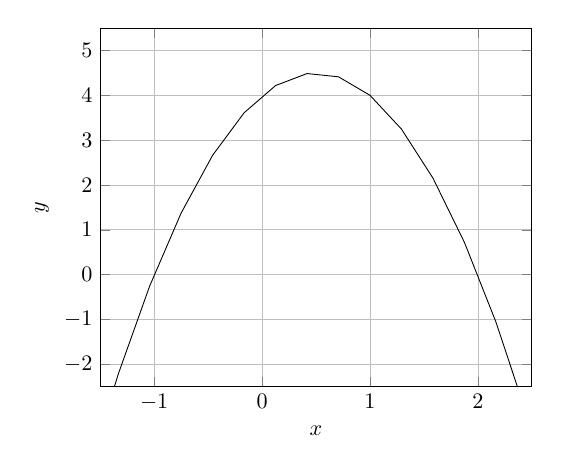
\begin{tikzpicture}[scale=0.8]
\begin{axis}[grid=both,
xmin=-1.5,xmax=2.5,
ymin=-2.5,ymax=5.5,
xtick={-2,...,4},
ytick={-4,...,5},
minor tick={},
xlabel=\(x\), ylabel=\(y\),
]
\addplot[domain=-2.5:4.5] {-2*(x+1)*(x-2)};
\end{axis}
\end{tikzpicture}
\end{center}

\end{exercise}


\begin{solution}
    $f(x)=-2(x+1)(x-2)$; $f(x)=-2x^2+2x+4$
\end{solution}



\begin{exercise} The graph of a quadratic function $g(t)$ is given below. Write the function in factored form. Then rewrite the function in standard form.

\begin{center}
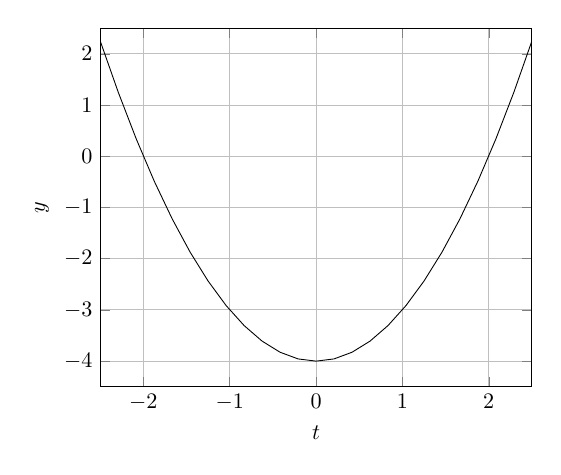
\begin{tikzpicture}[scale=0.8]
\begin{axis}[grid=both,
xmin=-2.5,xmax=2.5,
ymin=-4.5,ymax=2.5,
xtick={-2,...,2},
ytick={-4,...,2},
minor tick={},
xlabel=\(t\), ylabel=\(y\),
]
\addplot[domain=-2.5:2.5] {x^2-4};
\end{axis}
\end{tikzpicture}
\end{center}

\end{exercise}


\begin{solution}
    $g(t)=(t-2)(t+2)$; $g(t)=t^2-4$
\end{solution}

